
% Default to the notebook output style

    


% Inherit from the specified cell style.




    
\documentclass[11pt]{article}

    
    
    \usepackage[T1]{fontenc}
    % Nicer default font (+ math font) than Computer Modern for most use cases
    \usepackage{mathpazo}

    % Basic figure setup, for now with no caption control since it's done
    % automatically by Pandoc (which extracts ![](path) syntax from Markdown).
    \usepackage{graphicx}
    % We will generate all images so they have a width \maxwidth. This means
    % that they will get their normal width if they fit onto the page, but
    % are scaled down if they would overflow the margins.
    \makeatletter
    \def\maxwidth{\ifdim\Gin@nat@width>\linewidth\linewidth
    \else\Gin@nat@width\fi}
    \makeatother
    \let\Oldincludegraphics\includegraphics
    % Set max figure width to be 80% of text width, for now hardcoded.
    \renewcommand{\includegraphics}[1]{\Oldincludegraphics[width=.8\maxwidth]{#1}}
    % Ensure that by default, figures have no caption (until we provide a
    % proper Figure object with a Caption API and a way to capture that
    % in the conversion process - todo).
    \usepackage{caption}
    \DeclareCaptionLabelFormat{nolabel}{}
    \captionsetup{labelformat=nolabel}

    \usepackage{adjustbox} % Used to constrain images to a maximum size 
    \usepackage{xcolor} % Allow colors to be defined
    \usepackage{enumerate} % Needed for markdown enumerations to work
    \usepackage{geometry} % Used to adjust the document margins
    \usepackage{amsmath} % Equations
    \usepackage{amssymb} % Equations
    \usepackage{textcomp} % defines textquotesingle
    % Hack from http://tex.stackexchange.com/a/47451/13684:
    \AtBeginDocument{%
        \def\PYZsq{\textquotesingle}% Upright quotes in Pygmentized code
    }
    \usepackage{upquote} % Upright quotes for verbatim code
    \usepackage{eurosym} % defines \euro
    \usepackage[mathletters]{ucs} % Extended unicode (utf-8) support
    \usepackage[utf8x]{inputenc} % Allow utf-8 characters in the tex document
    \usepackage{fancyvrb} % verbatim replacement that allows latex
    \usepackage{grffile} % extends the file name processing of package graphics 
                         % to support a larger range 
    % The hyperref package gives us a pdf with properly built
    % internal navigation ('pdf bookmarks' for the table of contents,
    % internal cross-reference links, web links for URLs, etc.)
    \usepackage{hyperref}
    \usepackage{longtable} % longtable support required by pandoc >1.10
    \usepackage{booktabs}  % table support for pandoc > 1.12.2
    \usepackage[inline]{enumitem} % IRkernel/repr support (it uses the enumerate* environment)
    \usepackage[normalem]{ulem} % ulem is needed to support strikethroughs (\sout)
                                % normalem makes italics be italics, not underlines
    

    
    
    % Colors for the hyperref package
    \definecolor{urlcolor}{rgb}{0,.145,.698}
    \definecolor{linkcolor}{rgb}{.71,0.21,0.01}
    \definecolor{citecolor}{rgb}{.12,.54,.11}

    % ANSI colors
    \definecolor{ansi-black}{HTML}{3E424D}
    \definecolor{ansi-black-intense}{HTML}{282C36}
    \definecolor{ansi-red}{HTML}{E75C58}
    \definecolor{ansi-red-intense}{HTML}{B22B31}
    \definecolor{ansi-green}{HTML}{00A250}
    \definecolor{ansi-green-intense}{HTML}{007427}
    \definecolor{ansi-yellow}{HTML}{DDB62B}
    \definecolor{ansi-yellow-intense}{HTML}{B27D12}
    \definecolor{ansi-blue}{HTML}{208FFB}
    \definecolor{ansi-blue-intense}{HTML}{0065CA}
    \definecolor{ansi-magenta}{HTML}{D160C4}
    \definecolor{ansi-magenta-intense}{HTML}{A03196}
    \definecolor{ansi-cyan}{HTML}{60C6C8}
    \definecolor{ansi-cyan-intense}{HTML}{258F8F}
    \definecolor{ansi-white}{HTML}{C5C1B4}
    \definecolor{ansi-white-intense}{HTML}{A1A6B2}

    % commands and environments needed by pandoc snippets
    % extracted from the output of `pandoc -s`
    \providecommand{\tightlist}{%
      \setlength{\itemsep}{0pt}\setlength{\parskip}{0pt}}
    \DefineVerbatimEnvironment{Highlighting}{Verbatim}{commandchars=\\\{\}}
    % Add ',fontsize=\small' for more characters per line
    \newenvironment{Shaded}{}{}
    \newcommand{\KeywordTok}[1]{\textcolor[rgb]{0.00,0.44,0.13}{\textbf{{#1}}}}
    \newcommand{\DataTypeTok}[1]{\textcolor[rgb]{0.56,0.13,0.00}{{#1}}}
    \newcommand{\DecValTok}[1]{\textcolor[rgb]{0.25,0.63,0.44}{{#1}}}
    \newcommand{\BaseNTok}[1]{\textcolor[rgb]{0.25,0.63,0.44}{{#1}}}
    \newcommand{\FloatTok}[1]{\textcolor[rgb]{0.25,0.63,0.44}{{#1}}}
    \newcommand{\CharTok}[1]{\textcolor[rgb]{0.25,0.44,0.63}{{#1}}}
    \newcommand{\StringTok}[1]{\textcolor[rgb]{0.25,0.44,0.63}{{#1}}}
    \newcommand{\CommentTok}[1]{\textcolor[rgb]{0.38,0.63,0.69}{\textit{{#1}}}}
    \newcommand{\OtherTok}[1]{\textcolor[rgb]{0.00,0.44,0.13}{{#1}}}
    \newcommand{\AlertTok}[1]{\textcolor[rgb]{1.00,0.00,0.00}{\textbf{{#1}}}}
    \newcommand{\FunctionTok}[1]{\textcolor[rgb]{0.02,0.16,0.49}{{#1}}}
    \newcommand{\RegionMarkerTok}[1]{{#1}}
    \newcommand{\ErrorTok}[1]{\textcolor[rgb]{1.00,0.00,0.00}{\textbf{{#1}}}}
    \newcommand{\NormalTok}[1]{{#1}}
    
    % Additional commands for more recent versions of Pandoc
    \newcommand{\ConstantTok}[1]{\textcolor[rgb]{0.53,0.00,0.00}{{#1}}}
    \newcommand{\SpecialCharTok}[1]{\textcolor[rgb]{0.25,0.44,0.63}{{#1}}}
    \newcommand{\VerbatimStringTok}[1]{\textcolor[rgb]{0.25,0.44,0.63}{{#1}}}
    \newcommand{\SpecialStringTok}[1]{\textcolor[rgb]{0.73,0.40,0.53}{{#1}}}
    \newcommand{\ImportTok}[1]{{#1}}
    \newcommand{\DocumentationTok}[1]{\textcolor[rgb]{0.73,0.13,0.13}{\textit{{#1}}}}
    \newcommand{\AnnotationTok}[1]{\textcolor[rgb]{0.38,0.63,0.69}{\textbf{\textit{{#1}}}}}
    \newcommand{\CommentVarTok}[1]{\textcolor[rgb]{0.38,0.63,0.69}{\textbf{\textit{{#1}}}}}
    \newcommand{\VariableTok}[1]{\textcolor[rgb]{0.10,0.09,0.49}{{#1}}}
    \newcommand{\ControlFlowTok}[1]{\textcolor[rgb]{0.00,0.44,0.13}{\textbf{{#1}}}}
    \newcommand{\OperatorTok}[1]{\textcolor[rgb]{0.40,0.40,0.40}{{#1}}}
    \newcommand{\BuiltInTok}[1]{{#1}}
    \newcommand{\ExtensionTok}[1]{{#1}}
    \newcommand{\PreprocessorTok}[1]{\textcolor[rgb]{0.74,0.48,0.00}{{#1}}}
    \newcommand{\AttributeTok}[1]{\textcolor[rgb]{0.49,0.56,0.16}{{#1}}}
    \newcommand{\InformationTok}[1]{\textcolor[rgb]{0.38,0.63,0.69}{\textbf{\textit{{#1}}}}}
    \newcommand{\WarningTok}[1]{\textcolor[rgb]{0.38,0.63,0.69}{\textbf{\textit{{#1}}}}}
    
    
    % Define a nice break command that doesn't care if a line doesn't already
    % exist.
    \def\br{\hspace*{\fill} \\* }
    % Math Jax compatability definitions
    \def\gt{>}
    \def\lt{<}
    % Document parameters
    \title{Writeup}
    
    
    

    % Pygments definitions
    
\makeatletter
\def\PY@reset{\let\PY@it=\relax \let\PY@bf=\relax%
    \let\PY@ul=\relax \let\PY@tc=\relax%
    \let\PY@bc=\relax \let\PY@ff=\relax}
\def\PY@tok#1{\csname PY@tok@#1\endcsname}
\def\PY@toks#1+{\ifx\relax#1\empty\else%
    \PY@tok{#1}\expandafter\PY@toks\fi}
\def\PY@do#1{\PY@bc{\PY@tc{\PY@ul{%
    \PY@it{\PY@bf{\PY@ff{#1}}}}}}}
\def\PY#1#2{\PY@reset\PY@toks#1+\relax+\PY@do{#2}}

\expandafter\def\csname PY@tok@kd\endcsname{\let\PY@bf=\textbf\def\PY@tc##1{\textcolor[rgb]{0.00,0.50,0.00}{##1}}}
\expandafter\def\csname PY@tok@il\endcsname{\def\PY@tc##1{\textcolor[rgb]{0.40,0.40,0.40}{##1}}}
\expandafter\def\csname PY@tok@sr\endcsname{\def\PY@tc##1{\textcolor[rgb]{0.73,0.40,0.53}{##1}}}
\expandafter\def\csname PY@tok@mh\endcsname{\def\PY@tc##1{\textcolor[rgb]{0.40,0.40,0.40}{##1}}}
\expandafter\def\csname PY@tok@nd\endcsname{\def\PY@tc##1{\textcolor[rgb]{0.67,0.13,1.00}{##1}}}
\expandafter\def\csname PY@tok@vc\endcsname{\def\PY@tc##1{\textcolor[rgb]{0.10,0.09,0.49}{##1}}}
\expandafter\def\csname PY@tok@bp\endcsname{\def\PY@tc##1{\textcolor[rgb]{0.00,0.50,0.00}{##1}}}
\expandafter\def\csname PY@tok@cp\endcsname{\def\PY@tc##1{\textcolor[rgb]{0.74,0.48,0.00}{##1}}}
\expandafter\def\csname PY@tok@cm\endcsname{\let\PY@it=\textit\def\PY@tc##1{\textcolor[rgb]{0.25,0.50,0.50}{##1}}}
\expandafter\def\csname PY@tok@ch\endcsname{\let\PY@it=\textit\def\PY@tc##1{\textcolor[rgb]{0.25,0.50,0.50}{##1}}}
\expandafter\def\csname PY@tok@mo\endcsname{\def\PY@tc##1{\textcolor[rgb]{0.40,0.40,0.40}{##1}}}
\expandafter\def\csname PY@tok@s\endcsname{\def\PY@tc##1{\textcolor[rgb]{0.73,0.13,0.13}{##1}}}
\expandafter\def\csname PY@tok@kc\endcsname{\let\PY@bf=\textbf\def\PY@tc##1{\textcolor[rgb]{0.00,0.50,0.00}{##1}}}
\expandafter\def\csname PY@tok@kr\endcsname{\let\PY@bf=\textbf\def\PY@tc##1{\textcolor[rgb]{0.00,0.50,0.00}{##1}}}
\expandafter\def\csname PY@tok@ss\endcsname{\def\PY@tc##1{\textcolor[rgb]{0.10,0.09,0.49}{##1}}}
\expandafter\def\csname PY@tok@o\endcsname{\def\PY@tc##1{\textcolor[rgb]{0.40,0.40,0.40}{##1}}}
\expandafter\def\csname PY@tok@go\endcsname{\def\PY@tc##1{\textcolor[rgb]{0.53,0.53,0.53}{##1}}}
\expandafter\def\csname PY@tok@cpf\endcsname{\let\PY@it=\textit\def\PY@tc##1{\textcolor[rgb]{0.25,0.50,0.50}{##1}}}
\expandafter\def\csname PY@tok@gr\endcsname{\def\PY@tc##1{\textcolor[rgb]{1.00,0.00,0.00}{##1}}}
\expandafter\def\csname PY@tok@fm\endcsname{\def\PY@tc##1{\textcolor[rgb]{0.00,0.00,1.00}{##1}}}
\expandafter\def\csname PY@tok@ge\endcsname{\let\PY@it=\textit}
\expandafter\def\csname PY@tok@gd\endcsname{\def\PY@tc##1{\textcolor[rgb]{0.63,0.00,0.00}{##1}}}
\expandafter\def\csname PY@tok@c1\endcsname{\let\PY@it=\textit\def\PY@tc##1{\textcolor[rgb]{0.25,0.50,0.50}{##1}}}
\expandafter\def\csname PY@tok@err\endcsname{\def\PY@bc##1{\setlength{\fboxsep}{0pt}\fcolorbox[rgb]{1.00,0.00,0.00}{1,1,1}{\strut ##1}}}
\expandafter\def\csname PY@tok@vi\endcsname{\def\PY@tc##1{\textcolor[rgb]{0.10,0.09,0.49}{##1}}}
\expandafter\def\csname PY@tok@ne\endcsname{\let\PY@bf=\textbf\def\PY@tc##1{\textcolor[rgb]{0.82,0.25,0.23}{##1}}}
\expandafter\def\csname PY@tok@vg\endcsname{\def\PY@tc##1{\textcolor[rgb]{0.10,0.09,0.49}{##1}}}
\expandafter\def\csname PY@tok@nl\endcsname{\def\PY@tc##1{\textcolor[rgb]{0.63,0.63,0.00}{##1}}}
\expandafter\def\csname PY@tok@vm\endcsname{\def\PY@tc##1{\textcolor[rgb]{0.10,0.09,0.49}{##1}}}
\expandafter\def\csname PY@tok@mb\endcsname{\def\PY@tc##1{\textcolor[rgb]{0.40,0.40,0.40}{##1}}}
\expandafter\def\csname PY@tok@kp\endcsname{\def\PY@tc##1{\textcolor[rgb]{0.00,0.50,0.00}{##1}}}
\expandafter\def\csname PY@tok@sx\endcsname{\def\PY@tc##1{\textcolor[rgb]{0.00,0.50,0.00}{##1}}}
\expandafter\def\csname PY@tok@sc\endcsname{\def\PY@tc##1{\textcolor[rgb]{0.73,0.13,0.13}{##1}}}
\expandafter\def\csname PY@tok@nb\endcsname{\def\PY@tc##1{\textcolor[rgb]{0.00,0.50,0.00}{##1}}}
\expandafter\def\csname PY@tok@gs\endcsname{\let\PY@bf=\textbf}
\expandafter\def\csname PY@tok@gu\endcsname{\let\PY@bf=\textbf\def\PY@tc##1{\textcolor[rgb]{0.50,0.00,0.50}{##1}}}
\expandafter\def\csname PY@tok@nn\endcsname{\let\PY@bf=\textbf\def\PY@tc##1{\textcolor[rgb]{0.00,0.00,1.00}{##1}}}
\expandafter\def\csname PY@tok@mi\endcsname{\def\PY@tc##1{\textcolor[rgb]{0.40,0.40,0.40}{##1}}}
\expandafter\def\csname PY@tok@nv\endcsname{\def\PY@tc##1{\textcolor[rgb]{0.10,0.09,0.49}{##1}}}
\expandafter\def\csname PY@tok@sb\endcsname{\def\PY@tc##1{\textcolor[rgb]{0.73,0.13,0.13}{##1}}}
\expandafter\def\csname PY@tok@si\endcsname{\let\PY@bf=\textbf\def\PY@tc##1{\textcolor[rgb]{0.73,0.40,0.53}{##1}}}
\expandafter\def\csname PY@tok@dl\endcsname{\def\PY@tc##1{\textcolor[rgb]{0.73,0.13,0.13}{##1}}}
\expandafter\def\csname PY@tok@nc\endcsname{\let\PY@bf=\textbf\def\PY@tc##1{\textcolor[rgb]{0.00,0.00,1.00}{##1}}}
\expandafter\def\csname PY@tok@sa\endcsname{\def\PY@tc##1{\textcolor[rgb]{0.73,0.13,0.13}{##1}}}
\expandafter\def\csname PY@tok@sd\endcsname{\let\PY@it=\textit\def\PY@tc##1{\textcolor[rgb]{0.73,0.13,0.13}{##1}}}
\expandafter\def\csname PY@tok@gh\endcsname{\let\PY@bf=\textbf\def\PY@tc##1{\textcolor[rgb]{0.00,0.00,0.50}{##1}}}
\expandafter\def\csname PY@tok@ow\endcsname{\let\PY@bf=\textbf\def\PY@tc##1{\textcolor[rgb]{0.67,0.13,1.00}{##1}}}
\expandafter\def\csname PY@tok@gi\endcsname{\def\PY@tc##1{\textcolor[rgb]{0.00,0.63,0.00}{##1}}}
\expandafter\def\csname PY@tok@k\endcsname{\let\PY@bf=\textbf\def\PY@tc##1{\textcolor[rgb]{0.00,0.50,0.00}{##1}}}
\expandafter\def\csname PY@tok@gp\endcsname{\let\PY@bf=\textbf\def\PY@tc##1{\textcolor[rgb]{0.00,0.00,0.50}{##1}}}
\expandafter\def\csname PY@tok@nt\endcsname{\let\PY@bf=\textbf\def\PY@tc##1{\textcolor[rgb]{0.00,0.50,0.00}{##1}}}
\expandafter\def\csname PY@tok@kt\endcsname{\def\PY@tc##1{\textcolor[rgb]{0.69,0.00,0.25}{##1}}}
\expandafter\def\csname PY@tok@mf\endcsname{\def\PY@tc##1{\textcolor[rgb]{0.40,0.40,0.40}{##1}}}
\expandafter\def\csname PY@tok@sh\endcsname{\def\PY@tc##1{\textcolor[rgb]{0.73,0.13,0.13}{##1}}}
\expandafter\def\csname PY@tok@m\endcsname{\def\PY@tc##1{\textcolor[rgb]{0.40,0.40,0.40}{##1}}}
\expandafter\def\csname PY@tok@cs\endcsname{\let\PY@it=\textit\def\PY@tc##1{\textcolor[rgb]{0.25,0.50,0.50}{##1}}}
\expandafter\def\csname PY@tok@gt\endcsname{\def\PY@tc##1{\textcolor[rgb]{0.00,0.27,0.87}{##1}}}
\expandafter\def\csname PY@tok@na\endcsname{\def\PY@tc##1{\textcolor[rgb]{0.49,0.56,0.16}{##1}}}
\expandafter\def\csname PY@tok@s1\endcsname{\def\PY@tc##1{\textcolor[rgb]{0.73,0.13,0.13}{##1}}}
\expandafter\def\csname PY@tok@nf\endcsname{\def\PY@tc##1{\textcolor[rgb]{0.00,0.00,1.00}{##1}}}
\expandafter\def\csname PY@tok@kn\endcsname{\let\PY@bf=\textbf\def\PY@tc##1{\textcolor[rgb]{0.00,0.50,0.00}{##1}}}
\expandafter\def\csname PY@tok@s2\endcsname{\def\PY@tc##1{\textcolor[rgb]{0.73,0.13,0.13}{##1}}}
\expandafter\def\csname PY@tok@no\endcsname{\def\PY@tc##1{\textcolor[rgb]{0.53,0.00,0.00}{##1}}}
\expandafter\def\csname PY@tok@c\endcsname{\let\PY@it=\textit\def\PY@tc##1{\textcolor[rgb]{0.25,0.50,0.50}{##1}}}
\expandafter\def\csname PY@tok@w\endcsname{\def\PY@tc##1{\textcolor[rgb]{0.73,0.73,0.73}{##1}}}
\expandafter\def\csname PY@tok@ni\endcsname{\let\PY@bf=\textbf\def\PY@tc##1{\textcolor[rgb]{0.60,0.60,0.60}{##1}}}
\expandafter\def\csname PY@tok@se\endcsname{\let\PY@bf=\textbf\def\PY@tc##1{\textcolor[rgb]{0.73,0.40,0.13}{##1}}}

\def\PYZbs{\char`\\}
\def\PYZus{\char`\_}
\def\PYZob{\char`\{}
\def\PYZcb{\char`\}}
\def\PYZca{\char`\^}
\def\PYZam{\char`\&}
\def\PYZlt{\char`\<}
\def\PYZgt{\char`\>}
\def\PYZsh{\char`\#}
\def\PYZpc{\char`\%}
\def\PYZdl{\char`\$}
\def\PYZhy{\char`\-}
\def\PYZsq{\char`\'}
\def\PYZdq{\char`\"}
\def\PYZti{\char`\~}
% for compatibility with earlier versions
\def\PYZat{@}
\def\PYZlb{[}
\def\PYZrb{]}
\makeatother


    % Exact colors from NB
    \definecolor{incolor}{rgb}{0.0, 0.0, 0.5}
    \definecolor{outcolor}{rgb}{0.545, 0.0, 0.0}



    
    % Prevent overflowing lines due to hard-to-break entities
    \sloppy 
    % Setup hyperref package
    \hypersetup{
      breaklinks=true,  % so long urls are correctly broken across lines
      colorlinks=true,
      urlcolor=urlcolor,
      linkcolor=linkcolor,
      citecolor=citecolor,
      }
    % Slightly bigger margins than the latex defaults
    
    \geometry{verbose,tmargin=1in,bmargin=1in,lmargin=1in,rmargin=1in}
    
    

    \begin{document}
    
    
    \maketitle
    
    

    
    \hypertarget{traffic-sign-recognition}{%
\section{\texorpdfstring{\textbf{Traffic Sign
Recognition}}{Traffic Sign Recognition}}\label{traffic-sign-recognition}}

\hypertarget{writeup}{%
\subsection{Writeup}\label{writeup}}

\begin{center}\rule{0.5\linewidth}{\linethickness}\end{center}

\textbf{Build a Traffic Sign Recognition Project}

The goals / steps of this project are the following: * Load the data set
(see below for links to the project data set) * Explore, summarize and
visualize the data set * Design, train and test a model architecture *
Use the model to make predictions on new images * Analyze the softmax
probabilities of the new images * Summarize the results with a written
report

\hypertarget{rubric-points}{%
\subsection{Rubric Points}\label{rubric-points}}

\hypertarget{here-i-will-consider-the-rubric-points-individually-and-describe-how-i-addressed-each-point-in-my-implementation.}{%
\subsubsection{\texorpdfstring{Here I will consider the
\href{https://review.udacity.com/\#!/rubrics/481/view}{rubric points}
individually and describe how I addressed each point in my
implementation.}{Here I will consider the rubric points individually and describe how I addressed each point in my implementation.}}\label{here-i-will-consider-the-rubric-points-individually-and-describe-how-i-addressed-each-point-in-my-implementation.}}

\hypertarget{data-set-summary-exploration}{%
\subsubsection{Data Set Summary \&
Exploration}\label{data-set-summary-exploration}}

\hypertarget{provide-a-basic-summary-of-the-data-set.-in-the-code-the-analysis-should-be-done-using-python-numpy-andor-pandas-methods-rather-than-hardcoding-results-manually.}{%
\paragraph{1. Provide a basic summary of the data set. In the code, the
analysis should be done using python, numpy and/or pandas methods rather
than hardcoding results
manually.}\label{provide-a-basic-summary-of-the-data-set.-in-the-code-the-analysis-should-be-done-using-python-numpy-andor-pandas-methods-rather-than-hardcoding-results-manually.}}

I used the pandas library to calculate summary statistics of the traffic
signs data set:

\begin{itemize}
\tightlist
\item
  The size of training set is 34799
\item
  The size of the validation set is 4410
\item
  The size of test set is 12630
\item
  The shape of a traffic sign image is (32,32,3)
\item
  The number of unique classes/labels in the data set is 43
\end{itemize}

\hypertarget{include-an-exploratory-visualization-of-the-dataset.}{%
\paragraph{2. Include an exploratory visualization of the
dataset.}\label{include-an-exploratory-visualization-of-the-dataset.}}

Here is an exploratory visualization of the data set. It is a bar chart
showing how the data is divided as training and validation images. It
shows the number of samples of each class on the traning set and the
validation set.

\begin{figure}
\centering
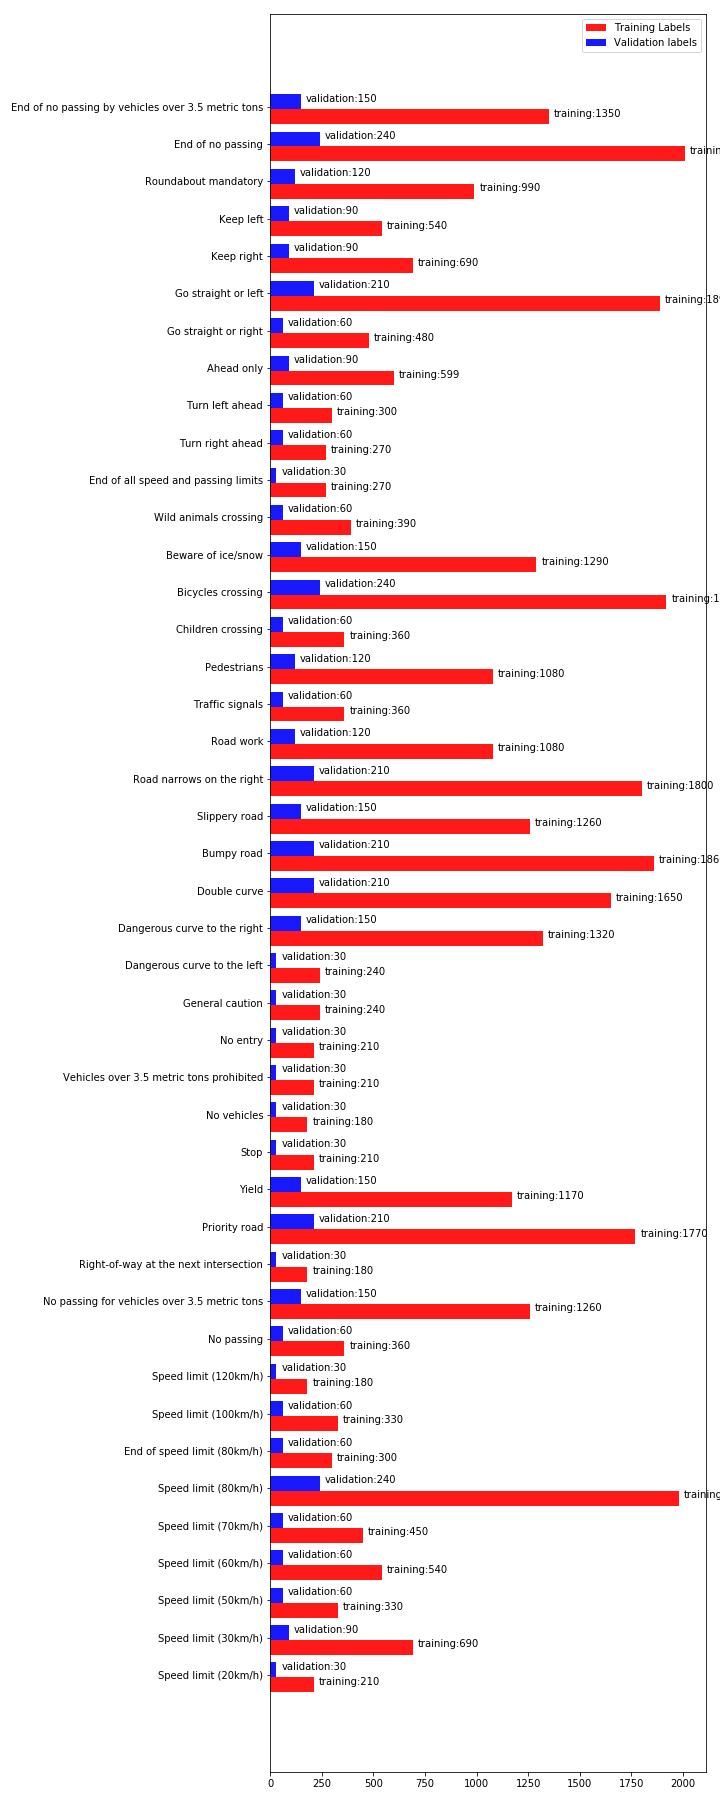
\includegraphics{./examples/visualization.png}
\caption{alt text}
\end{figure}

\hypertarget{design-and-test-a-model-architecture}{%
\subsubsection{Design and Test a Model
Architecture}\label{design-and-test-a-model-architecture}}

\hypertarget{describe-how-you-preprocessed-the-image-data.-what-techniques-were-chosen-and-why-did-you-choose-these-techniques-consider-including-images-showing-the-output-of-each-preprocessing-technique.-pre-processing-refers-to-techniques-such-as-converting-to-grayscale-normalization-etc.-optional-as-described-in-the-stand-out-suggestions-part-of-the-rubric-if-you-generated-additional-data-for-training-describe-why-you-decided-to-generate-additional-data-how-you-generated-the-data-and-provide-example-images-of-the-additional-data.-then-describe-the-characteristics-of-the-augmented-training-set-like-number-of-images-in-the-set-number-of-images-for-each-class-etc.}{%
\paragraph{1. Describe how you preprocessed the image data. What
techniques were chosen and why did you choose these techniques? Consider
including images showing the output of each preprocessing technique.
Pre-processing refers to techniques such as converting to grayscale,
normalization, etc. (OPTIONAL: As described in the ``Stand Out
Suggestions'' part of the rubric, if you generated additional data for
training, describe why you decided to generate additional data, how you
generated the data, and provide example images of the additional data.
Then describe the characteristics of the augmented training set like
number of images in the set, number of images for each class,
etc.)}\label{describe-how-you-preprocessed-the-image-data.-what-techniques-were-chosen-and-why-did-you-choose-these-techniques-consider-including-images-showing-the-output-of-each-preprocessing-technique.-pre-processing-refers-to-techniques-such-as-converting-to-grayscale-normalization-etc.-optional-as-described-in-the-stand-out-suggestions-part-of-the-rubric-if-you-generated-additional-data-for-training-describe-why-you-decided-to-generate-additional-data-how-you-generated-the-data-and-provide-example-images-of-the-additional-data.-then-describe-the-characteristics-of-the-augmented-training-set-like-number-of-images-in-the-set-number-of-images-for-each-class-etc.}}

I split the data using train\_test\_split() from
sklearn.model\_selection library. I have choosen 20\% as test\_size.\\
Then,I normalized the image data because I want the image data to be in
the range from 0 to 1. I have used ImageDataGenerator from
Keras.preprocessing.image library to preprocess the data and augment it
in real time. My ImageDataGenerator() argument values are given below

\begin{verbatim}
     | Argument                     |      Value               |
     |:----------------------------:|:------------------------:|
     |featurewise_center            |     False                |
     |featurewise_std_normalization |     False                |
     |shear_range                   |     0.1                  |
     |rotation_range                |     10.0                 |
     |width_shift_range             |     0.1                  |
     |height_shift_range            |     0.1                  |
     |zoom_range                    |     0.2                  |
     
\end{verbatim}

\hypertarget{describe-what-your-final-model-architecture-looks-like-including-model-type-layers-layer-sizes-connectivity-etc.-consider-including-a-diagram-andor-table-describing-the-final-model.}{%
\paragraph{2. Describe what your final model architecture looks like
including model type, layers, layer sizes, connectivity, etc.) Consider
including a diagram and/or table describing the final
model.}\label{describe-what-your-final-model-architecture-looks-like-including-model-type-layers-layer-sizes-connectivity-etc.-consider-including-a-diagram-andor-table-describing-the-final-model.}}

I have used Keras.Sequential to design my model architecture. Sequential
is a keras container fot linear stack of layers. Layers will do
automatic shape inference expect the first layer, In the first layer I
have provided the input shape as (32,32,3).

I have designed a model with 6 convolutional layers and a fully
connected layer. I have added one dropout layer to prevent overfitting.
My output contains a softmax activation function to return the
probabilties.

My final model consisted of the following layers:

\begin{longtable}[]{@{}cc@{}}
\toprule
Layer & Description\tabularnewline
\midrule
\endhead
Input & 32x32x3 RGB image\tabularnewline
Convolution 1 & 3x3 kernel, SAME padding, 32 Filters,relu
activation\tabularnewline
Convolution 2 & 3x3 kernel, SAME padding, 32 Filters,relu
activation\tabularnewline
Max pooling & 2x2 stride, VALID padding\tabularnewline
Convolution 3 & 3x3 kernel, SAME padding, 64 Filters,relu
activation\tabularnewline
Convolution 4 & 3x3 kernel, SAME padding, 64 Filters,relu
activation\tabularnewline
Max pooling & 2x2 stride, VALID padding\tabularnewline
Convolution 5 & 3x3 kernel, SAME padding, 128 Filters,relu
activation\tabularnewline
Convolution 6 & 3x3 kernel, SAME padding, 128 Filters,relu
activation\tabularnewline
Max pooling & 2x2 stride, VALID padding\tabularnewline
Flatten &\tabularnewline
Dense 1 & Outputs 512, relu activation\tabularnewline
dropout & Keep\_prob=0.5\tabularnewline
Dense 2 & Outputs 43, softmax activation\tabularnewline
\bottomrule
\end{longtable}

To train the model, I have used `categorical\_crossentropy' as my loss
fucntion, `stochastic gradient descent(SGD)' as optimizer and metric is
`accuracy' and compiled the model using keras model.compile().

While Training the model I have generated more data on the fly by keras
preprocessing techniques. I have used LearningRateScheduler from
keras.callbacks library to select decaying learning rate over the
epochs. I have used below function to decay the learning over the
epochs. def learning\_rate(epoch): return 0.001*(0.1**int(epoch/10))

I have trained the model using below function in keras

model.fit\_generator(datagen.flow(X\_train,y\_train,batch\_size=batch\_size),steps\_per\_epoch=1500,epochs=epochs,validation\_data=(X\_validation,y\_validation)
, callbacks={[}LearningRateScheduler(lr\_schedule),
ModelCheckpoint(`model.h5',save\_best\_only=True){]})

Hyper parameters used in the model are given below

\begin{longtable}[]{@{}cc@{}}
\toprule
HyperParameter & Value\tabularnewline
\midrule
\endhead
Epochs & 10\tabularnewline
Batch Size & 32\tabularnewline
Learning rate & 0.001\tabularnewline
Keep\_Prob & 0.5\tabularnewline
\bottomrule
\end{longtable}

First, my parameters are like- Constant learning rate=0.001,
epochs=30,batch\_size=32,
steps\_per\_epoch=X\_train.shape{[}0{]}//batch\_size, and I had 3
dropout layers in my CNN. With this setup I have got a validation
accuracy of 90.65\%.

Later, I used decaying learning rate, epochs=10, batch\_size=64, and
removed two dropout layers, My validation accuarcy was 94.87\%

When I set the steps\_per\_epoch=X\_train.shape{[}0{]} and It took a lot
of time to train the model.

After trying different values for parameters, finally I have used
decaying learning rate, epochs=10, Batch\_size=32,
steps\_per\_epoch=1500, I have got a validation accuracy of 98.38\%

My final model results were: * training set accuracy of 95.00\% *
validation set accuracy of 98.38\%

Below I have provided the Learning curves
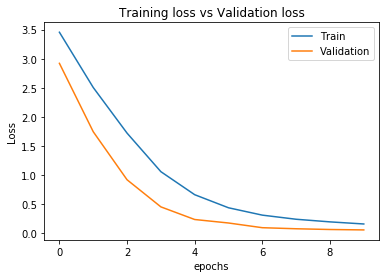
\includegraphics{./learning_curve.PNG}

\hypertarget{test-a-model-on-new-images}{%
\subsubsection{Test a Model on New
Images}\label{test-a-model-on-new-images}}

\hypertarget{choose-five-german-traffic-signs-found-on-the-web-and-provide-them-in-the-report.-for-each-image-discuss-what-quality-or-qualities-might-be-difficult-to-classify.}{%
\paragraph{1. Choose five German traffic signs found on the web and
provide them in the report. For each image, discuss what quality or
qualities might be difficult to
classify.}\label{choose-five-german-traffic-signs-found-on-the-web-and-provide-them-in-the-report.-for-each-image-discuss-what-quality-or-qualities-might-be-difficult-to-classify.}}

Here are six German traffic signs that I found on the web:

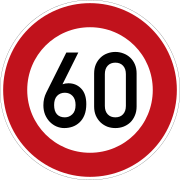
\includegraphics{./test_image/60.png}
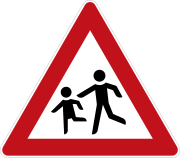
\includegraphics{./test_image/Children.png}

\includegraphics{./test_image/stop.png}
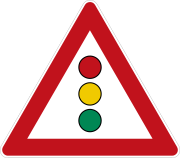
\includegraphics{./test_image/Traffic.png}
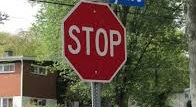
\includegraphics{./test_image/tiltedSTOP.jpg}
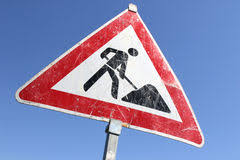
\includegraphics{./test_image/Rw1.jpg}

The first four images are colored opaque images so I converted them to 3
channel(RGB) images. The last two images might be difficult to classify
because the STOP sign is tilted at angle when it is resized to (32,32)
it has become more noisy, And the Road work sign in not clear and also
tilted.

Since I have added more image data by preprocessing the images while
trianing my model is able to identify thes images correctly. Without
data augmentation It may be difficult to identify the signs in these two
images.

\hypertarget{discuss-the-models-predictions-on-these-new-traffic-signs-and-compare-the-results-to-predicting-on-the-test-set.-at-a-minimum-discuss-what-the-predictions-were-the-accuracy-on-these-new-predictions-and-compare-the-accuracy-to-the-accuracy-on-the-test-set-optional-discuss-the-results-in-more-detail-as-described-in-the-stand-out-suggestions-part-of-the-rubric.}{%
\paragraph{2. Discuss the model's predictions on these new traffic signs
and compare the results to predicting on the test set. At a minimum,
discuss what the predictions were, the accuracy on these new
predictions, and compare the accuracy to the accuracy on the test set
(OPTIONAL: Discuss the results in more detail as described in the
``Stand Out Suggestions'' part of the
rubric).}\label{discuss-the-models-predictions-on-these-new-traffic-signs-and-compare-the-results-to-predicting-on-the-test-set.-at-a-minimum-discuss-what-the-predictions-were-the-accuracy-on-these-new-predictions-and-compare-the-accuracy-to-the-accuracy-on-the-test-set-optional-discuss-the-results-in-more-detail-as-described-in-the-stand-out-suggestions-part-of-the-rubric.}}

Here are the results of the prediction:

\begin{longtable}[]{@{}cc@{}}
\toprule
Image & Prediction\tabularnewline
\midrule
\endhead
Speed limit (60km/h) & Speed limit (60km/h)\tabularnewline
Children crossing & Children crossing\tabularnewline
Traffic signals & Traffic signals\tabularnewline
Stop & Stop\tabularnewline
Road work & Roadwork\tabularnewline
tilted STOP & STOP\tabularnewline
\bottomrule
\end{longtable}

The model was able to correctly guess all the 7 traffic signs, which
gives an accuracy of 100\%.

\hypertarget{describe-how-certain-the-model-is-when-predicting-on-each-of-the-five-new-images-by-looking-at-the-softmax-probabilities-for-each-prediction.-provide-the-top-5-softmax-probabilities-for-each-image-along-with-the-sign-type-of-each-probability.-optional-as-described-in-the-stand-out-suggestions-part-of-the-rubric-visualizations-can-also-be-provided-such-as-bar-charts}{%
\paragraph{3. Describe how certain the model is when predicting on each
of the five new images by looking at the softmax probabilities for each
prediction. Provide the top 5 softmax probabilities for each image along
with the sign type of each probability. (OPTIONAL: as described in the
``Stand Out Suggestions'' part of the rubric, visualizations can also be
provided such as bar
charts)}\label{describe-how-certain-the-model-is-when-predicting-on-each-of-the-five-new-images-by-looking-at-the-softmax-probabilities-for-each-prediction.-provide-the-top-5-softmax-probabilities-for-each-image-along-with-the-sign-type-of-each-probability.-optional-as-described-in-the-stand-out-suggestions-part-of-the-rubric-visualizations-can-also-be-provided-such-as-bar-charts}}

The top five probalities for each test image is given below.
Probabilties are 1 for all the test images except for 60 speed limit the
accuracy was 99.445\%.

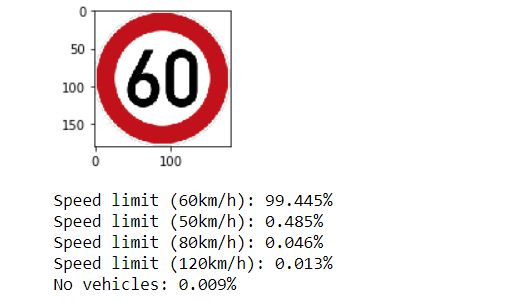
\includegraphics{./snipped/1.PNG} 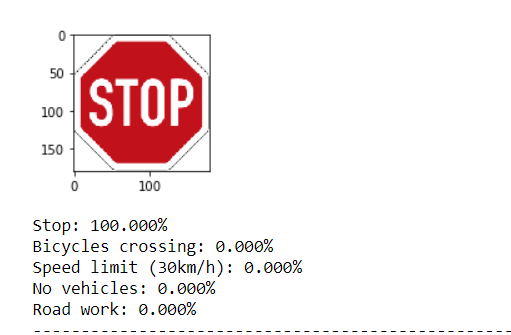
\includegraphics{./snipped/5.PNG}
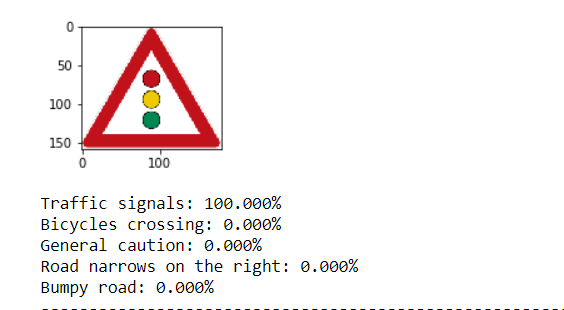
\includegraphics{./snipped/3.PNG} 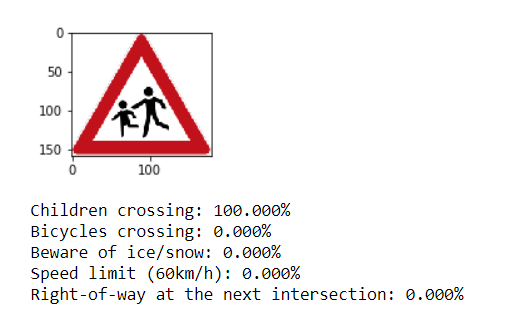
\includegraphics{./snipped/2.PNG}
{[}alt text{]}{[}image17{]} 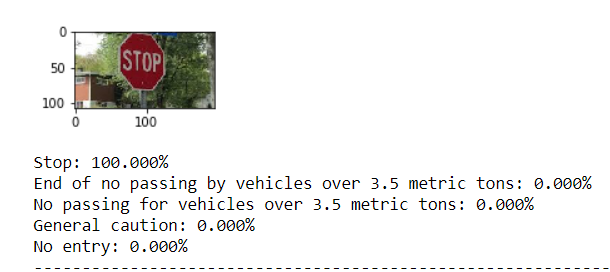
\includegraphics{./snipped/6.PNG}
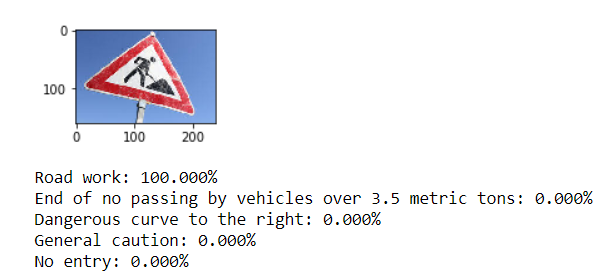
\includegraphics{./snipped/4.PNG}


    % Add a bibliography block to the postdoc
    
    
    
    \end{document}
